\documentclass[a4paper,11pt]{article}
\usepackage[utf8]{inputenc}
\usepackage[margin=0.8in]{geometry}
\usepackage{tikz}
\usepackage{graphicx}
\usetikzlibrary{arrows.meta}

\begin{document}

\section*{Historical and Structural Analysis: Mestre's Evolution}

\begin{tikzpicture}[x=1cm, y=1.2cm]
    % Vertical Arrow (Thick and Red)
    \draw[->, ultra thick, -{Latex[length=6mm]}, red!80!black] (0,0.5) -- (0,-15);

    % Timeline Nodes with Labels
    \node[anchor=west] at (0.3, 0) {\textbf{1917–70}: Industrialization of Porto Marghera};
    \node[anchor=west] at (0.3, -1.3) {\textbf{1926}: Annexation to Venezia};
    \node[anchor=west] at (0.3, -2.6) {\textbf{1959–61}: PRG Dorigo Moratorium};
    \node[anchor=west] at (0.3, -3.9) {\textbf{1972}: Tangenziale A57};
    \node[anchor=west] at (0.3, -5.2) {\textbf{1960s-90s}: Suburban Sprawl};
    \node[anchor=west] at (0.3, -6.5) {\textbf{1997}: Piazza Ferretto Restyling};
    \node[anchor=west] at (0.3, -7.8) {\textbf{2004}: Parco San Giuliano};
    \node[anchor=west] at (0.3, -9.1) {\textbf{2004}: Master Plan Marghera};
    \node[anchor=west] at (0.3, -10.4) {\textbf{2018}: M9 Museum};
    \node[anchor=west] at (0.3, -11.7) {\textbf{2026}: New Station Hub};

    % Insert first 3 images (using placeholders as requested in the workflow)
    \node[anchor=west] at (8, -0.5) {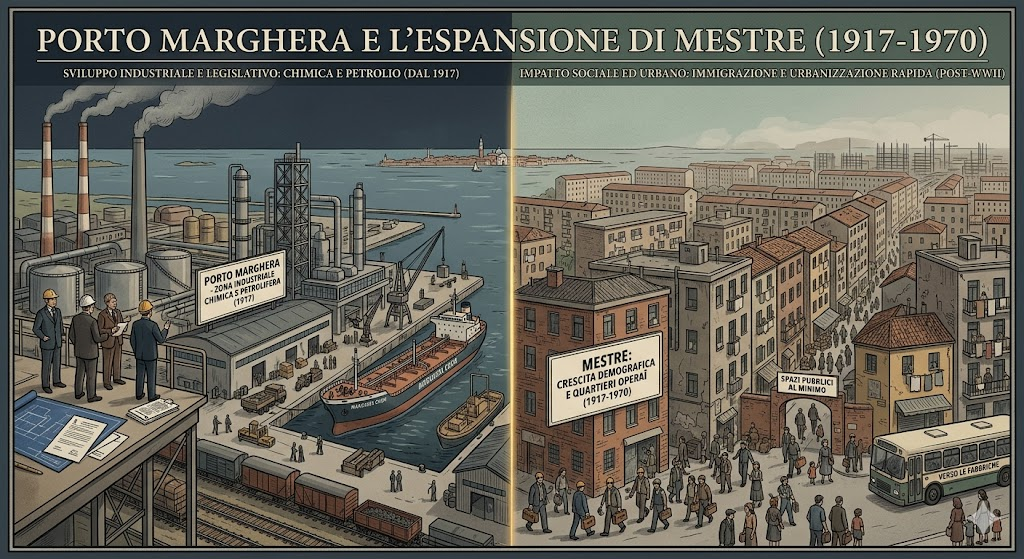
\includegraphics[width=3cm]{image/1917-1970.jpeg}};
    \node[anchor=west] at (8, -2.5) {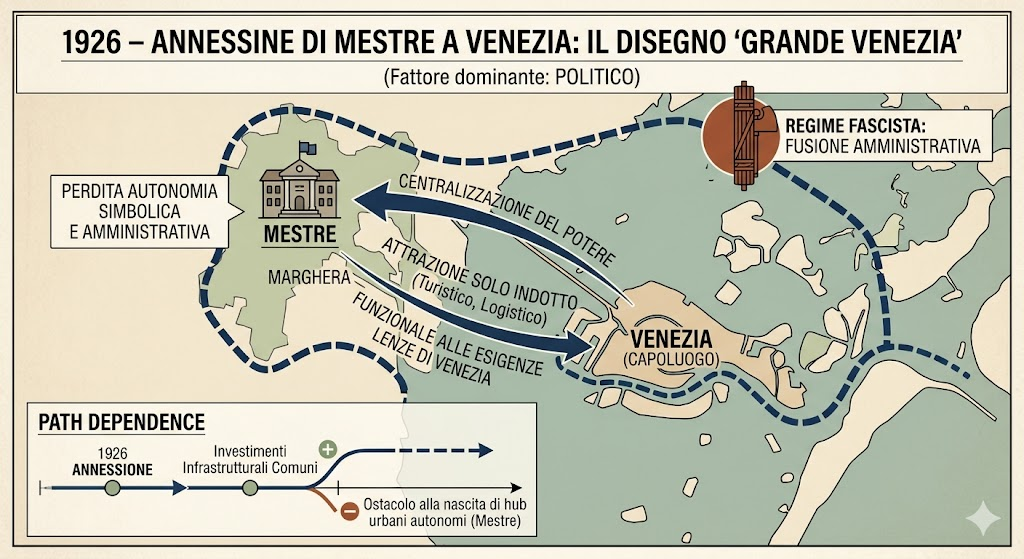
\includegraphics[width=3cm]{image/1926 Annessione.jpeg}};
    \node[anchor=west] at (8, -4.5) {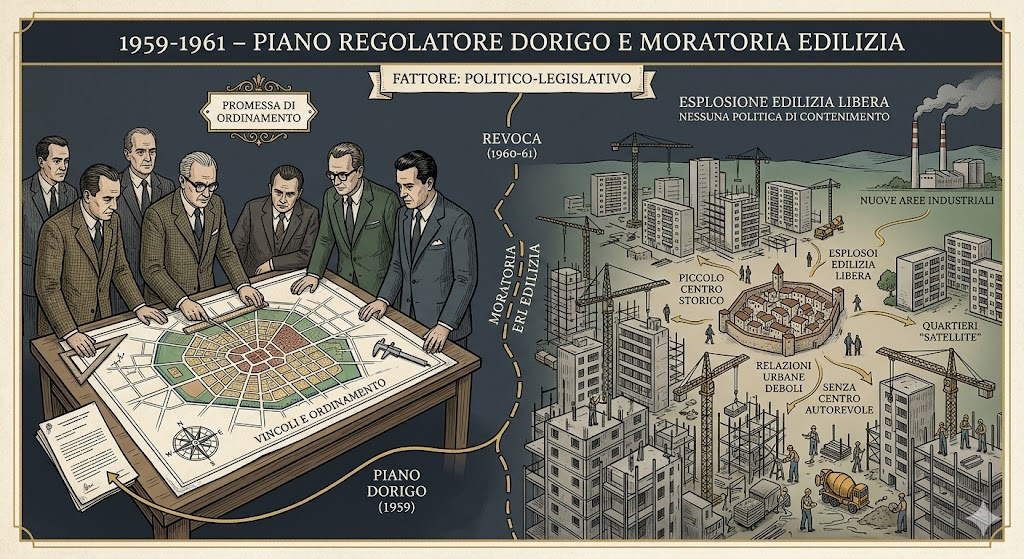
\includegraphics[width=3cm]{image/1959-1961.jpeg}};
\end{tikzpicture}

\newpage

\section*{Evolutionary Analysis and Structural Determinants}

\subsection*{The Founding Moment: Industrialization (1917–1970)}
The systemic trajectory originates here. This is the causal beginning that established Mestre’s demographic mass and its monofunctional economic dependency, creating a rigid structure that regeneration efforts still struggle to overcome.

\subsection*{Critical Events \& Lock-in Factors}
\begin{itemize}
    \item \textbf{1926 Annexation (Political Lock-in):} An irreversible administrative choice. By surrendering autonomous civic status, Mestre became a subordinate functional periphery, permanently hindering independent urban identity.
    \item \textbf{1959–61 PRG Dorigo/Moratorium (Legal Irreversibility):} The choice not to impose strict zoning led to chaotic, low-density sprawl. This "freedom of expansion" is now a rigid constraint, leaving the city without a central nervous system.
    \item \textbf{1972 Tangenziale A57 (Infrastructural Lock-in):} A technological lock-in. This infrastructure cemented the "city of transit" model, creating physical barriers that today discourage the pedestrian walkability required for social hubs.
\end{itemize}

\subsection*{Systemic Trap: The "Flagship" Strategy}
Current decision-makers favor "flagship" projects (M9 Museum, Parco San Giuliano, New Station). These represent a \textbf{Systemic Trap}:
\begin{itemize}
    \item \textbf{Why it's a trap:} Flagships are top-down, predictable, and politically visible. They avoid the structural compromise of density and social mix required for true urban intelligence.
    \item \textbf{The Trade-off:} Prioritizing isolated landmarks maintains systemic rigidity. True regeneration would require a \textit{diffused network of places}, which demands higher social investment with less immediate political return.
\end{itemize}

\end{document}
